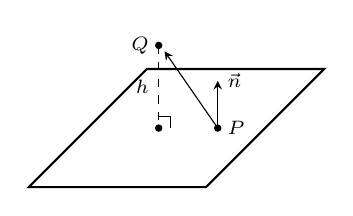
\begin{tikzpicture}[scale=1.5,>=stealth]
	\draw [thick] (0,0) -- (1,1) -- (2.5,1) -- (1.5,0) -- cycle;
	
	\filldraw (1.6,.5) circle (.75pt) node [right] {\scriptsize $P$}
						(1.1,1.2) circle (.75pt) node [left] {\scriptsize $Q$};
	\draw [->] (1.6,.5) -- (1.6,.9) node [right] {\scriptsize$\vec n$};
	\draw [->] (1.6,.5) -- (1.15,1.15);% node [right] {\scriptsize$\vec n$};
	\draw [dashed] (1.1,1.2) -- (1.1,.5) node [pos=.5,left] {\scriptsize $h$};
	\filldraw (1.1,.5) circle (.75pt);
	\draw (1.1,.6) -- (1.2,.6) -- (1.2,.5);
	%\draw 
	
\end{tikzpicture}
